\documentclass[11pt,a4paper]{article}

\usepackage[T1]{fontenc}
\usepackage[utf8]{inputenc}
\usepackage[a4paper,margin=2.1cm]{geometry}
\usepackage{amsmath,amssymb,mathtools,bm}
\usepackage{array}
\usepackage{booktabs}
\usepackage{longtable}
\usepackage{tabularx}
\usepackage{xcolor}
\usepackage{graphicx}
\usepackage{tikz}
\usetikzlibrary{arrows.meta,calc,positioning,shapes.geometric}
\usepackage{enumitem}
\usepackage{listings}
\usepackage{hyperref}
\usepackage[strings]{underscore}

\hypersetup{
  colorlinks=true,
  linkcolor=blue!50!black,
  urlcolor=blue!50!black
}

\definecolor{brand}{RGB}{18,71,122}
\definecolor{accent}{RGB}{0,116,97}
\definecolor{warn}{RGB}{172,72,36}
\definecolor{soft}{RGB}{247,249,252}
\definecolor{line}{RGB}{210,218,230}
\definecolor{textgray}{RGB}{82,90,105}
\definecolor{codebg}{RGB}{246,248,250}

\lstdefinestyle{cppstyle}{
  language=C++,
  basicstyle=\ttfamily\small,
  backgroundcolor=\color{codebg},
  frame=single,
  rulecolor=\color{line},
  breaklines=true,
  columns=fullflexible,
  keywordstyle=\color{brand}\bfseries,
  commentstyle=\color{textgray},
  stringstyle=\color{accent!80!black},
  showstringspaces=false
}

\lstset{style=cppstyle}

\newcommand{\code}[1]{\ifmmode\text{\ttfamily\detokenize{#1}}\else\texttt{\detokenize{#1}}\fi}
\newcommand{\pkg}{\code{auto_aim}}
\newcommand{\repo}{\code{auto_aim_complete_refactor}}
\newcommand{\vect}[1]{\bm{#1}}
\newcommand{\mat}[1]{\mathbf{#1}}
\newcommand{\R}{\mathbb{R}}

\newenvironment{studybox}[1]
{\par\medskip\noindent\fcolorbox{brand!35}{soft}{\begin{minipage}{0.96\linewidth}\textbf{\color{brand}#1}\par\smallskip}}
{\end{minipage}\par\medskip}

\newenvironment{warningbox}[1]
{\par\medskip\noindent\fcolorbox{warn!45}{warn!5}{\begin{minipage}{0.96\linewidth}\textbf{\color{warn}#1}\par\smallskip}}
{\end{minipage}\par\medskip}

\title{\vspace{-1.0cm}\textbf{\repo: Mathematics And Code Course}\\
\large From algebra basics to the exact EKF, PnP, ballistics, ROS callbacks, and command behavior in your new auto-aim code}
\author{Generated from the workspace source code}
\date{Source snapshot studied on May 7, 2026}

\begin{document}
\maketitle

\begin{center}
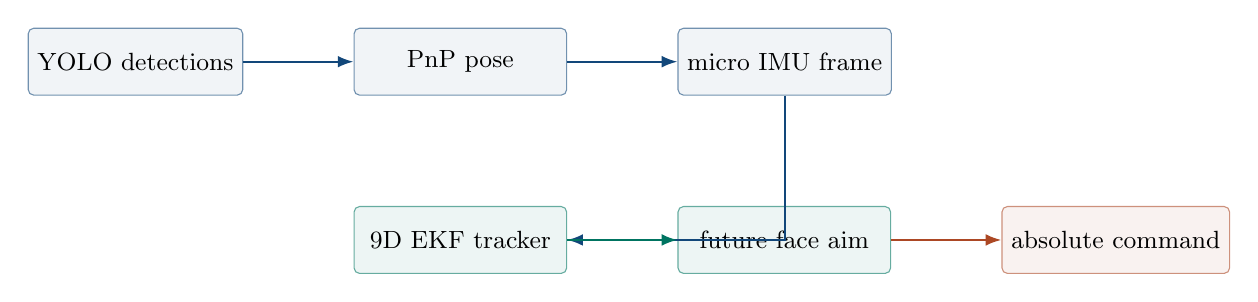
\begin{tikzpicture}[node distance=1.4cm, every node/.style={font=\small}]
  \node[draw=brand!60, fill=brand!6, rounded corners=2pt, minimum width=2.7cm, minimum height=0.85cm] (det) {YOLO detections};
  \node[draw=brand!60, fill=brand!6, rounded corners=2pt, right=of det, minimum width=2.7cm, minimum height=0.85cm] (pnp) {PnP pose};
  \node[draw=brand!60, fill=brand!6, rounded corners=2pt, right=of pnp, minimum width=2.7cm, minimum height=0.85cm] (tf) {micro IMU frame};
  \node[draw=accent!60, fill=accent!7, rounded corners=2pt, below=of pnp, minimum width=2.7cm, minimum height=0.85cm] (ekf) {9D EKF tracker};
  \node[draw=accent!60, fill=accent!7, rounded corners=2pt, right=of ekf, minimum width=2.7cm, minimum height=0.85cm] (aim) {future face aim};
  \node[draw=warn!60, fill=warn!7, rounded corners=2pt, right=of aim, minimum width=2.7cm, minimum height=0.85cm] (cmd) {absolute command};
  \draw[-{Latex[length=2mm]}, thick, color=brand] (det) -- (pnp);
  \draw[-{Latex[length=2mm]}, thick, color=brand] (pnp) -- (tf);
  \draw[-{Latex[length=2mm]}, thick, color=brand] (tf) |- (ekf);
  \draw[-{Latex[length=2mm]}, thick, color=accent] (ekf) -- (aim);
  \draw[-{Latex[length=2mm]}, thick, color=warn] (aim) -- (cmd);
\end{tikzpicture}
\end{center}

\tableofcontents
\clearpage

\section{How To Study This Document}

This file is a course for the ignored root package \repo, whose ROS package name is \pkg.
The source files used are:
\begin{itemize}[leftmargin=1.4em]
  \item \path{auto_aim_complete_refactor/src/auto_aim_node.cpp}
  \item \path{auto_aim_complete_refactor/src/tracker.cpp}
  \item \path{auto_aim_complete_refactor/include/auto_aim/tracker.hpp}
  \item \path{auto_aim_complete_refactor/src/pnp_solver.cpp}
  \item \path{auto_aim_complete_refactor/include/auto_aim/pnp_solver.hpp}
  \item \path{auto_aim_complete_refactor/launch/auto_aim_launch.py}
\end{itemize}

\begin{studybox}{Main idea}
Your code does not simply point the gimbal at the middle of a YOLO box.
It converts 2D boxes into 3D armor measurements, transforms those measurements into the same reference used by the microcontroller, filters them with an Extended Kalman Filter, predicts which armor face will be hittable when the bullet arrives, compensates gravity and barrel offset, then publishes absolute yaw and pitch commands.
\end{studybox}

The course starts from the smallest math ideas because EKF notation can look intimidating if algebra, vectors, matrices, trigonometry, and probability are not already comfortable.
Read it in order the first time.
After that, use the glossary and code mapping tables as reference.

\section{Vocabulary Before The Math}

\begin{longtable}{p{0.24\linewidth} p{0.70\linewidth}}
\toprule
\textbf{Word} & \textbf{Meaning in this project} \\
\midrule
\endfirsthead
\toprule
\textbf{Word} & \textbf{Meaning in this project} \\
\midrule
\endhead
Detection & A 2D object found by YOLO. In your code it arrives on \code{/detector/armors} as a \code{vision_msgs::msg::Detection2DArray}. \\
Bounding box & A rectangle in the image around an armor plate. It has center pixel \((c_x,c_y)\), width \(w\), and height \(h\). \\
PnP & Perspective-n-Point. A computer vision method that estimates a 3D pose from known 3D model points and their 2D image positions. \\
Pose & Position plus orientation. Position says where something is. Orientation says how it is rotated. \\
Frame & A coordinate system. A point like \((1,2,3)\) means nothing unless we know the frame. \\
Odom & A world-like reference frame used by the tracker and RViz markers. In this refactor it is built manually from the micro yaw and pitch, not through a full TF lookup chain. \\
IMU & Inertial measurement unit. Here \code{/micro_imu} is a \code{Float32MultiArray} carrying current yaw and pitch from the lower computer. \\
Tracker & The object that remembers a target over time. Your tracker stores a 9D state vector and a 9x9 covariance matrix. \\
EKF & Extended Kalman Filter. A filter for estimating hidden state when the equations are nonlinear. \\
State & The internal variables the tracker believes describe the target: center position, velocities, yaw, yaw rate, and radius. \\
Measurement & What the sensors report this frame: armor position and armor yaw. \\
Prediction & What the tracker thinks will happen before seeing the next measurement. \\
Update & The correction step where the measurement pulls the prediction closer to reality. \\
Covariance & A matrix describing uncertainty. Big diagonal entries mean the tracker is unsure. Off-diagonal entries mean two errors are statistically related. \\
Ballistics & The math of projectile flight. Your refactor models gravity, not drag. \\
Fire gate & Logic deciding whether the robot may fire now. \\
Hysteresis & A small memory effect that prevents a boolean from flickering on and off near a threshold. \\
\bottomrule
\end{longtable}

\section{Algebra Basics}

\subsection{Numbers, Variables, And Units}

A \textbf{number} is a value such as \(3\), \(0.05\), or \(\pi\).
A \textbf{variable} is a name for a value that can change, such as:
\[
  dt,\quad r,\quad x_c,\quad v_x,\quad \psi.
\]
In robotics, units matter.
Your code mostly uses:
\begin{itemize}[leftmargin=1.4em]
  \item meters for distance;
  \item seconds for time;
  \item radians for angles;
  \item meters per second for linear velocity;
  \item radians per second for angular velocity.
\end{itemize}

\begin{studybox}{Unit check}
The equation \(x_{\text{new}} = x + v\,dt\) is valid because
\[
  \text{meters} = \text{meters} + \frac{\text{meters}}{\text{second}}\cdot \text{second}.
\]
Always check units when an equation feels suspicious.
\end{studybox}

\subsection{Functions}

A \textbf{function} maps an input to an output:
\[
  y = f(x).
\]
Example:
\[
  f(x) = x^2,\qquad f(3)=9.
\]

In your tracker, the EKF uses two important functions:
\[
  \vect{x}_{k+1} = f(\vect{x}_k)
  \qquad\text{and}\qquad
  \vect{z}_k = h(\vect{x}_k).
\]
The first is the \textbf{process model}: it predicts the next target state.
The second is the \textbf{observation model}: it predicts what measurement the camera should see if the state were correct.

\subsection{Linear Versus Nonlinear}

A \textbf{linear} equation has only scaling and addition.
For example:
\[
  y = 2x + 3.
\]
The graph is a straight line.

A \textbf{nonlinear} equation includes operations such as sine, cosine, multiplication between variables, powers, or divisions:
\[
  y = r\cos(\psi).
\]
Your observation model is nonlinear because the armor position depends on \(\cos(\psi)\) and \(\sin(\psi)\).
This is exactly why the code uses an Extended Kalman Filter instead of a plain Kalman Filter.

\section{Vectors And Matrices}

\subsection{Vectors}

A \textbf{vector} is an ordered list of numbers.
The EKF state is a vector:
\[
\vect{x} =
\begin{bmatrix}
x_c & v_{x_c} & y_c & v_{y_c} & z_a & v_{z_a} & \psi & \dot{\psi} & r
\end{bmatrix}^{T}.
\]
The superscript \(T\) means transpose, so the row shown above is really a column:
\[
\vect{x} =
\begin{bmatrix}
x_c\\
v_{x_c}\\
y_c\\
v_{y_c}\\
z_a\\
v_{z_a}\\
\psi\\
\dot{\psi}\\
r
\end{bmatrix}.
\]

\begin{longtable}{p{0.18\linewidth} p{0.74\linewidth}}
\toprule
\textbf{Symbol} & \textbf{Meaning} \\
\midrule
\endfirsthead
\toprule
\textbf{Symbol} & \textbf{Meaning} \\
\midrule
\endhead
\(x_c\) & Target center \(x\) coordinate in the tracker frame. \\
\(v_{x_c}\) & Target center velocity along \(x\). \\
\(y_c\) & Target center \(y\) coordinate in the tracker frame. \\
\(v_{y_c}\) & Target center velocity along \(y\). \\
\(z_a\) & Height of the currently modeled armor face. The code names it \code{za}. \\
\(v_{z_a}\) & Vertical velocity estimate for \(z_a\). \\
\(\psi\) & Target yaw. In this refactor it follows the inward-facing armor convention. \\
\(\dot{\psi}\) & Yaw rate, meaning how fast the target is spinning. \\
\(r\) & Orbit radius from target center to armor plate. \\
\bottomrule
\end{longtable}

\subsection{Matrices}

A \textbf{matrix} is a rectangular table of numbers.
The covariance matrix \(P\) is \(9\times 9\), meaning 9 rows and 9 columns.
The observation Jacobian \(H\) is \(4\times 9\), because it maps 9 state variables into 4 measurement variables.

\subsection{Matrix Multiplication}

If \(\mat{A}\) is \(m\times n\) and \(\vect{x}\) is \(n\times 1\), then \(\mat{A}\vect{x}\) is \(m\times 1\).
The inner dimensions must match:
\[
  (m\times n)(n\times 1) = (m\times 1).
\]

This matters in the Kalman gain:
\[
  \mat{K} = \mat{P}\mat{H}^{T}\mat{S}^{-1}.
\]
In your code:
\[
  \mat{P}:9\times 9,\quad
  \mat{H}^{T}:9\times 4,\quad
  \mat{S}^{-1}:4\times 4,
\]
so:
\[
  \mat{K}:9\times 4.
\]
That is correct because the gain converts a 4D measurement error into a 9D state correction.

\subsection{Norms And Distance}

A \textbf{norm} is a length.
For a 3D vector:
\[
  \|\vect{p}\| = \sqrt{x^2+y^2+z^2}.
\]
Your code uses this idea for:
\begin{itemize}[leftmargin=1.4em]
  \item detection range: \(\sqrt{x^2+y^2+z^2}\);
  \item ground distance: \(\sqrt{x^2+y^2}\);
  \item match distance: distance between predicted armor position and detected armor position.
\end{itemize}

\section{Trigonometry For Auto-Aim}

\subsection{Radians}

Robotics code almost always uses radians.
\[
  180^\circ = \pi\ \text{rad},\qquad
  90^\circ = \frac{\pi}{2}\ \text{rad}.
\]
Your commands are published as absolute radians in a \code{Twist}, even though the custom \code{GimbalCmd.msg} comments mention relative degrees.

\begin{warningbox}{Code reality}
The custom message file \path{auto_aim_complete_refactor/msg/GimbalCmd.msg} says yaw and pitch are relative degrees.
The node actually publishes \code{geometry_msgs::msg::Twist} on \code{/tracker/cmd_gimbal} and \code{/cmd_vel_AI}, with absolute yaw and pitch in radians in the microcontroller convention.
\end{warningbox}

\subsection{Sine, Cosine, And Circular Motion}

For an angle \(\psi\), a point on a circle of radius \(r\) has coordinates:
\[
  x = r\cos\psi,\qquad y = r\sin\psi.
\]
Your armor model uses the reverse direction because the armor is offset from the center:
\[
  x_a = x_c - r\cos\psi,\qquad
  y_a = y_c - r\sin\psi.
\]

\begin{center}
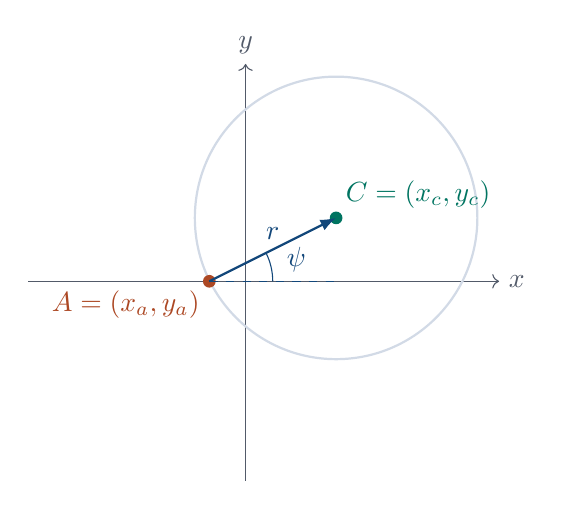
\begin{tikzpicture}[scale=2.3]
  \draw[->, color=textgray] (-1.2,0) -- (1.4,0) node[right] {$x$};
  \draw[->, color=textgray] (0,-1.1) -- (0,1.2) node[above] {$y$};
  \coordinate (C) at (0.5,0.35);
  \coordinate (A) at ($(C)+(-0.7,-0.35)$);
  \draw[color=line, thick] (C) circle (0.78);
  \fill[color=accent] (C) circle (0.035) node[above right] {$C=(x_c,y_c)$};
  \fill[color=warn] (A) circle (0.035) node[below left] {$A=(x_a,y_a)$};
  \draw[-{Latex[length=2mm]}, thick, color=brand] (A) -- (C) node[midway, above] {$r$};
  \draw[dashed, color=brand] (A) -- ($(A)+(0.7,0)$);
  \draw[color=brand] ($(A)+(0.35,0)$) arc[start angle=0,end angle=26.565,radius=0.35];
  \node[color=brand] at ($(A)+(0.48,0.12)$) {$\psi$};
\end{tikzpicture}
\end{center}

\subsection{\texorpdfstring{\(\texttt{atan2}\)}{atan2}}

\code{atan2(y,x)} returns the angle of the vector \((x,y)\).
It is safer than \(\arctan(y/x)\) because it knows which quadrant the vector is in.
Your code uses it for:
\[
  \text{bearing} = \operatorname{atan2}(y,x).
\]
\textbf{Bearing} means the yaw angle from the origin or barrel to a target point.

\subsection{Shortest Angular Distance}

Angles wrap around.
For example, \(179^\circ\) and \(-179^\circ\) are only \(2^\circ\) apart, not \(358^\circ\).
The code uses \code{angles::shortest_angular_distance(a,b)} to compute the smallest signed rotation from \(a\) to \(b\).

This is used in:
\begin{itemize}[leftmargin=1.4em]
  \item yaw unwrapping;
  \item target yaw jump detection;
  \item yaw command smoothing across \(-\pi/\pi\);
  \item fire-window error.
\end{itemize}

\section{Calculus: Derivatives And Jacobians}

\subsection{Derivative}

A \textbf{derivative} measures how fast one value changes when another value changes.
For example:
\[
  \frac{d}{dx}x^2 = 2x.
\]
In words: near a chosen \(x\), a small change \(\Delta x\) causes about \(2x\Delta x\) change in \(x^2\).

\subsection{Partial Derivative}

When a function has multiple inputs, a \textbf{partial derivative} asks how the output changes with one input while the others stay fixed.
For:
\[
  f(x,y)=x^2+3y,
\]
we have:
\[
  \frac{\partial f}{\partial x}=2x,\qquad
  \frac{\partial f}{\partial y}=3.
\]

\subsection{Jacobian}

A \textbf{Jacobian} is a matrix of partial derivatives.
The EKF needs Jacobians because it approximates nonlinear functions locally by linear ones.

If:
\[
  \vect{z} = h(\vect{x}),
\]
then:
\[
  \mat{H} = \frac{\partial h}{\partial \vect{x}}.
\]
Your code builds \(\mat{H}\) manually in \code{Tracker::ekfUpdate()} and \code{Tracker::ekfMahalanobis()}.

\section{Probability And Uncertainty}

\subsection{Mean}

The \textbf{mean} is the best estimate.
In the EKF, the state vector \(\vect{x}\) is the mean of the tracker's belief:
\[
  \text{best estimate} = \vect{x}.
\]

\subsection{Variance}

\textbf{Variance} measures uncertainty in one number.
Small variance means high confidence.
Large variance means low confidence.

The initial covariance in your code is:
\[
\operatorname{diag}(P_0)=
\begin{bmatrix}
0.1 & 1.0 & 0.1 & 1.0 & 0.1 & 0.2 & 0.1 & 3.0 & 0.01
\end{bmatrix}.
\]
The yaw-rate variance starts large because spin rate is hard to know from one detection.

\subsection{Covariance}

\textbf{Covariance} measures whether two errors tend to move together.
If \(x_c\) and \(v_{x_c}\) are correlated, an error in position also says something about velocity.

The covariance matrix \(P\) stores all variances and covariances:
\[
P =
\begin{bmatrix}
\sigma_{x_1}^2 & \sigma_{x_1x_2} & \cdots\\
\sigma_{x_2x_1} & \sigma_{x_2}^2 & \cdots\\
\vdots & \vdots & \ddots
\end{bmatrix}.
\]

\subsection{Gaussian Belief}

A \textbf{Gaussian} is the bell-curve distribution.
Kalman filters assume the current belief is approximately Gaussian:
\[
  \vect{x} \sim \mathcal{N}(\hat{\vect{x}}, P).
\]
This means:
\begin{itemize}[leftmargin=1.4em]
  \item \(\hat{\vect{x}}\) is the estimated state;
  \item \(P\) is the uncertainty around that estimate.
\end{itemize}

\section{Coordinate Frames And Camera Geometry}

\subsection{Frame Discipline}

The refactor avoids a large TF chain and instead uses the microcontroller yaw and pitch directly.
The input \code{/micro_imu} must contain:
\[
  \text{data}[0] = \text{yaw rad},\qquad
  \text{data}[1] = \text{pitch rad}.
\]
Then the node builds:
\[
  q_{\text{gimbal}} = \operatorname{RPY}(0,\theta,\psi),
\]
where \(\theta\) is pitch and \(\psi\) is yaw.
It also builds a camera optical conversion:
\[
  q_{\text{conv}} = \operatorname{RPY}\left(-\frac{\pi}{2},0,-\frac{\pi}{2}\right).
\]
The final rotation is:
\[
  q_{\text{imu}} = q_{\text{gimbal}}q_{\text{conv}}.
\]

For a point measured by PnP in the camera frame:
\[
  \vect{p}_{\text{odom}} =
  R(q_{\text{imu}})\vect{p}_{\text{cam}}
  +
  \begin{bmatrix}0\\0\\h_g\end{bmatrix}.
\]
In the code, \(h_g\) is \code{cfg_.gimbal_height}.

\begin{warningbox}{Important limitation}
The translation only uses gimbal height.
The refactor does not model a full camera mounting offset in this measurement transform.
Barrel offset is handled later in aiming, not here.
\end{warningbox}

\subsection{Camera Intrinsics}

A pinhole camera maps a 3D camera-frame point \((X,Y,Z)\) to image pixels:
\[
  u = f_x\frac{X}{Z}+c_x,\qquad
  v = f_y\frac{Y}{Z}+c_y.
\]
The matrix form is:
\[
K =
\begin{bmatrix}
f_x & 0 & c_x\\
0 & f_y & c_y\\
0 & 0 & 1
\end{bmatrix}.
\]
Your \code{PnPSolver::init()} receives this \(K\) from \code{/camera_info}.

\section{PnP In Your Code}

\subsection{The Armor Plate Model}

The PnP solver tries two physical armor sizes:
\[
  \text{small}: 140\text{ mm}\times 125\text{ mm},
  \qquad
  \text{large}: 235\text{ mm}\times 127\text{ mm}.
\]
The 3D points lie on a flat plate in object coordinates:
\[
\begin{bmatrix}
0 & +w/2 & -h/2\\
0 & +w/2 & +h/2\\
0 & -w/2 & +h/2\\
0 & -w/2 & -h/2
\end{bmatrix}.
\]
The \(x=0\) means the plate is modeled as a flat rectangle.

\subsection{Image Points From A Bounding Box}

The solver does not use detected light corners.
It constructs four image points from the bounding box:
\[
\begin{aligned}
l_x &= c_x - \lambda w/2, & r_x &= c_x + \lambda w/2,\\
t_y &= c_y - \lambda h/2, & b_y &= c_y + \lambda h/2,
\end{aligned}
\]
where \(\lambda = \code{light_ratio}\).
Then:
\[
  \{(l_x,b_y),(l_x,t_y),(r_x,t_y),(r_x,b_y)\}.
\]

\begin{studybox}{Why shrink the box?}
\code{light_ratio} shrinks the rectangle because the YOLO box may include padding or glow around the lights.
Using a slightly smaller rectangle can better approximate the real armor plate corners.
\end{studybox}

\subsection{Solving And Choosing Small Or Large}

For each model, the code calls:
\[
  \code{cv::solvePnP(..., SOLVEPNP_IPPE)}.
\]
Then it projects the 3D model points back into the image and computes average pixel error:
\[
  e = \frac{1}{4}\sum_{i=1}^{4}\|\vect{u}_i^{\text{projected}}-\vect{u}_i^{\text{input}}\|.
\]
This is called \textbf{reprojection error}.
The model with lower reprojection error wins, as long as the error is below \code{max_reproj_error}.

\subsection{Yaw Convention Correction}

PnP yaw can be flipped by \(180^\circ\), especially for a flat rectangle.
The refactor corrects this before passing the detection into the tracker.

The tracker expects \(\psi\) to point from the visible armor plate inward toward the enemy robot center.
For a visible front plate, this direction should roughly align with the bearing from your robot to the armor:
\[
  \psi_{\text{bearing}} = \operatorname{atan2}(y_{\text{odom}}, x_{\text{odom}}).
\]
The code does:
\begin{enumerate}[leftmargin=1.4em]
  \item if PnP yaw differs from bearing by more than \(90^\circ\), add \(\pi\);
  \item if it is still too oblique, replace yaw with the bearing itself.
\end{enumerate}

\begin{studybox}{Why this matters}
Without this correction, the observation model can put the estimated target center on the wrong side of the armor.
That is a filter-poisoning error: the EKF may be mathematically correct but correcting toward the wrong geometry.
\end{studybox}

\section{The Tracker State Machine}

\subsection{States}

Your tracker has four states:
\[
  \code{LOST},\quad \code{DETECTING},\quad \code{TRACKING},\quad \code{TEMP_LOST}.
\]

\begin{longtable}{p{0.18\linewidth} p{0.74\linewidth}}
\toprule
\textbf{State} & \textbf{Meaning} \\
\midrule
\endfirsthead
\toprule
\textbf{State} & \textbf{Meaning} \\
\midrule
\endhead
\code{LOST} & No valid target is currently tracked. If detections exist, the closest detection initializes the EKF. \\
\code{DETECTING} & A candidate target exists, but it needs \code{confirm_frames} successful matched frames before becoming trusted. \\
\code{TRACKING} & The target is confirmed. Aiming and fire decisions may happen. \\
\code{TEMP_LOST} & The tracker missed detections briefly but continues predicting for up to \code{lost_timeout}. \\
\bottomrule
\end{longtable}

\subsection{Target Switching}

The comments in the header describe an aggressive closest-target policy, but the actual \code{shouldSwitch()} code is conservative:
\begin{itemize}[leftmargin=1.4em]
  \item if \code{LOST}, any candidate can initialize;
  \item during \code{DETECTING} or \code{TRACKING}, it does not switch;
  \item during \code{TEMP_LOST}, it may switch only if cooldown is over and the new target is closer than \(\text{current range}\times\code{switch_range_ratio}\).
\end{itemize}

\begin{warningbox}{Code reality}
Study the implementation, not only the comments.
In the current source, the tracker does not drop a confirmed visible target just because a closer target appears.
\end{warningbox}

\section{The EKF: Big Picture}

\subsection{What The EKF Is Estimating}

The tracker keeps:
\[
\vect{x} =
\begin{bmatrix}
x_c\\v_{x_c}\\y_c\\v_{y_c}\\z_a\\v_{z_a}\\\psi\\\dot{\psi}\\r
\end{bmatrix}
\in \R^9,
\qquad
P\in\R^{9\times 9}.
\]
The measurement is:
\[
\vect{z} =
\begin{bmatrix}
x_a\\y_a\\z_a\\\psi_a
\end{bmatrix}
\in \R^4.
\]

The hidden target is not exactly the armor plate.
The state estimates the target center and spin, while the measurement observes one armor face.
That difference is the key to the whole tracker.

\subsection{Predict Then Update}

Every frame, after initialization, the tracker does:
\[
\text{predict} \rightarrow \text{associate} \rightarrow \text{update or coast}.
\]

\textbf{Predict} means advance the old state forward by \(dt\).
\textbf{Associate} means decide which detection, if any, matches the predicted target.
\textbf{Update} means fuse the matched detection into the EKF.
\textbf{Coast} means no detection matched, so the prediction remains the best estimate.

\section{EKF Predict Step In Your Code}

\subsection{Damped Constant-Velocity Model}

For each position-velocity pair, the model is:
\[
  p_{\text{new}} = p + v\,b\,dt,
  \qquad
  v_{\text{new}} = v\,b.
\]
For yaw:
\[
  \psi_{\text{new}} = \psi + \dot{\psi}\,a\,dt,
  \qquad
  \dot{\psi}_{\text{new}} = \dot{\psi}\,a.
\]

Here \(b\) is position damping and \(a\) is yaw damping:
\[
  b = \alpha_{\text{pos}}^{dt\,f_{\text{ref}}},
  \qquad
  a = \alpha_{\text{yaw}}^{dt\,f_{\text{ref}}}.
\]
During \code{TEMP_LOST}, both use:
\[
  \alpha_{\text{coast}}^{dt\,f_{\text{ref}}}.
\]

\begin{studybox}{Why damping is time-normalized}
If the camera runs at 30 Hz, \(dt f_{\text{ref}}=1\), so damping is exactly the configured alpha.
If the frame rate changes, the exponent keeps roughly the same damping per second rather than per frame.
\end{studybox}

\subsection{State Transition Matrix}

For one pair \([p,v]^T\), the Jacobian block is:
\[
\mat{F}_{pv} =
\begin{bmatrix}
1 & b\,dt\\
0 & b
\end{bmatrix}.
\]
So:
\[
\begin{bmatrix}
p_{\text{new}}\\
v_{\text{new}}
\end{bmatrix}
=
\begin{bmatrix}
1 & b\,dt\\
0 & b
\end{bmatrix}
\begin{bmatrix}
p\\
v
\end{bmatrix}.
\]
Your code puts this block into \(x,y,z\), and yaw/yaw-rate pairs.

\subsection{Process Noise}

\textbf{Process noise} means uncertainty caused by motion that the simple model cannot explain:
acceleration, slipping, impacts, irregular spinning, or timing error.

For each position-velocity pair, your code uses:
\[
\mat{Q}_{pv} =
\sigma^2
\begin{bmatrix}
\frac{dt^4}{4} & \frac{dt^3}{2}\\
\frac{dt^3}{2} & dt^2
\end{bmatrix}.
\]
This is the classic white-noise acceleration model.
The state covariance prediction is:
\[
  P \leftarrow \mat{F}P\mat{F}^T+\mat{Q}.
\]

\section{EKF Observation Model}

\subsection{From State To Expected Measurement}

The observed armor plate is offset from the target center:
\[
\begin{aligned}
x_a &= x_c-r\cos\psi,\\
y_a &= y_c-r\sin\psi,\\
z_a &= z_a,\\
\psi_a &= \psi.
\end{aligned}
\]
So:
\[
h(\vect{x}) =
\begin{bmatrix}
x_c-r\cos\psi\\
y_c-r\sin\psi\\
z_a\\
\psi
\end{bmatrix}.
\]

\subsection{Observation Jacobian}

Differentiate \(h(\vect{x})\) with respect to the 9 state variables.
The matrix used by your code is:
\[
\mat{H} =
\begin{bmatrix}
1&0&0&0&0&0&r\sin\psi&0&-\cos\psi\\
0&0&1&0&0&0&-r\cos\psi&0&-\sin\psi\\
0&0&0&0&1&0&0&0&0\\
0&0&0&0&0&0&1&0&0
\end{bmatrix}.
\]

The non-obvious terms are:
\[
\frac{\partial}{\partial\psi}(x_c-r\cos\psi)=r\sin\psi,
\]
\[
\frac{\partial}{\partial\psi}(y_c-r\sin\psi)=-r\cos\psi.
\]
These terms tell the EKF that yaw error can look like position error.

\section{Measurement Noise}

\subsection{Range-Dependent Noise}

PnP gets worse at long range.
The code sets:
\[
  \sigma_p = \code{r_pos_base} + \code{r_pos_slope}\cdot d,
\]
\[
  \sigma_\psi = \code{r_yaw_base} + \code{r_yaw_slope}\cdot d,
\]
where:
\[
  d = \sqrt{x_a^2+y_a^2+z_a^2}.
\]

\subsection{Obliquity}

\textbf{Obliquity} means how edge-on the armor plate is to the camera.
A face-on plate gives reliable yaw.
An edge-on plate gives unreliable yaw.

The code computes:
\[
  \phi = |\operatorname{shortest}(\psi_a,\operatorname{atan2}(y_a,x_a))|.
\]
Then:
\[
  c=\cos\phi.
\]
Position noise is multiplied by:
\[
  f_{xyz}=\frac{1}{\max(c^2,0.04)}.
\]
Yaw noise is multiplied by:
\[
  f_\psi=\frac{1}{\max(|c|^4,10^{-4})}.
\]
If \(\phi\) is larger than \code{max_oblique_deg}, yaw noise becomes huge:
\[
  f_\psi = 10^6.
\]
This does not delete the measurement.
It tells the EKF: use position, but almost ignore yaw.

\subsection{Measurement Covariance}

The measurement covariance matrix is:
\[
\mat{R} =
\begin{bmatrix}
\sigma_p^2 f_{xyz}&0&0&0\\
0&\sigma_p^2 f_{xyz}&0&0\\
0&0&\sigma_p^2 f_{xyz}&0\\
0&0&0&\sigma_\psi^2 f_{\psi}
\end{bmatrix}.
\]

\section{EKF Update Step}

\subsection{Innovation}

The \textbf{innovation} is the measurement residual:
\[
  \vect{y} = \vect{z}-h(\vect{x}).
\]
It means: what did the sensor see that the current prediction did not expect?

\subsection{Innovation Covariance}

\[
  \mat{S} = \mat{H}P\mat{H}^{T}+\mat{R}.
\]
\(\mat{S}\) combines uncertainty from the predicted state and uncertainty from the measurement.

\subsection{Kalman Gain}

\[
  \mat{K}=P\mat{H}^{T}\mat{S}^{-1}.
\]
The Kalman gain decides how strongly the measurement corrects the state.

If \(P\) is large and \(R\) is small, the tracker is unsure and the measurement is trusted more.
If \(P\) is small and \(R\) is large, the tracker is confident and the measurement is trusted less.

\subsection{State Correction}

\[
  \vect{x} \leftarrow \vect{x} + \mat{K}\vect{y}.
\]
This is the heart of the Kalman filter.

\subsection{Joseph Form Covariance Update}

Your code uses:
\[
  P \leftarrow
  (\mat{I}-\mat{K}\mat{H})P(\mat{I}-\mat{K}\mat{H})^{T}
  +
  \mat{K}\mat{R}\mat{K}^{T}.
\]
This is called the \textbf{Joseph form}.
It is more numerically stable than the shorter \(P\leftarrow(\mat{I}-\mat{K}\mat{H})P\).

\begin{studybox}{Positive semidefinite}
A covariance matrix must not contain physically impossible negative uncertainty.
Joseph form helps keep \(P\) symmetric and positive semidefinite despite floating-point roundoff.
\end{studybox}

\section{Mahalanobis Gating}

\subsection{Why Plain Distance Is Not Enough}

A detection can be rejected using Euclidean distance:
\[
  \|\vect{p}_{\text{pred}}-\vect{p}_{\text{det}}\|.
\]
But that ignores uncertainty.
If the tracker is very uncertain, a larger error might still be acceptable.
If the tracker is very certain, a small error might be suspicious.

\subsection{Mahalanobis Distance}

Mahalanobis distance is:
\[
  m = \vect{y}^{T}\mat{S}^{-1}\vect{y}.
\]
It measures error in units of expected uncertainty.
Your code accepts the best detection only if:
\[
  m < \code{maha_threshold}.
\]
The launch default is \(13.3\).
For a 4D measurement, this is roughly a high-confidence outlier gate.

\section{Armor Matching And Armor Jumps}

\subsection{Normal Match}

After prediction, the tracker searches detections with the same class id as the current target.
For each candidate it computes Mahalanobis distance.
The lowest candidate under the threshold wins.

Then it checks:
\[
  p_d < \code{max_match_dist}
\]
and either:
\[
  y_d < \code{yaw_jump_thresh}
\]
or the plate is oblique.
If so, it performs a normal EKF update.

\subsection{Yaw Jump}

If yaw changes too much and the plate is not oblique:
\[
  y_d > \code{yaw_jump_thresh},
\]
the tracker treats it as an \textbf{armor jump}.
This means the enemy rotated and a different face is now visible.

\subsection{Radius Swap And Height Offset}

For a 4-armor target, opposite pairs can have different radius or height.
When the jump angle is roughly \(90^\circ\), the code:
\begin{itemize}[leftmargin=1.4em]
  \item flips \code{dz_};
  \item updates \code{dz_} with a slow blend;
  \item swaps \code{radius_} and \code{other_radius_};
  \item resets vertical velocity.
\end{itemize}

\subsection{Divergence Reset}

After a jump, the code compares:
\[
  \|\vect{p}_{\text{inferred armor}}-\vect{p}_{\text{detected armor}}\|.
\]
If it is too large, the filter is considered divergent and the state is rebuilt directly from the detection:
\[
  x_c = x_a+r\cos\psi,\qquad
  y_c = y_a+r\sin\psi.
\]
Then \(P\) is reset to \(P_0\).

\section{Radius Estimation}

The state contains \(r\), but the code updates the stored radius with an exponential moving average:
\[
  r \leftarrow (1-\alpha)r+\alpha r_{\text{meas}}.
\]
The measured radius is:
\[
  r_{\text{meas}} =
  (x_c-x_a)\cos\psi + (y_c-y_a)\sin\psi.
\]
This projects the center-to-armor vector onto the yaw direction.
The update is skipped when the plate is too oblique, because oblique PnP geometry is unreliable.

\begin{studybox}{EMA}
EMA means Exponential Moving Average.
It is a simple smoother: small \(\alpha\) changes slowly, large \(\alpha\) reacts quickly.
The default \code{radius_ema_alpha} is \(0.05\), so radius adapts slowly.
\end{studybox}

\section{Ballistics}

\subsection{The Problem}

The camera and tracker estimate a target point.
The bullet does not travel in a perfectly straight line.
Gravity pulls it down.
Therefore the gimbal must aim higher than the direct line to the target.

\subsection{Gravity-Only Solver}

Given ground distance \(g_d\), vertical difference \(d_z\), and bullet speed \(v\), the code starts with:
\[
  \theta_0 = \operatorname{atan2}(d_z,g_d).
\]
Then it iterates five times:
\[
  v_x = v\cos\theta,
\]
\[
  t = \frac{g_d}{v_x},
\]
\[
  \theta \leftarrow
  \operatorname{atan2}\left(d_z+\frac{1}{2}gt^2,\ g_d\right).
\]
The \(+\frac{1}{2}gt^2\) term aims above the target by the expected gravity drop.

The final flight time is:
\[
  t_{\text{flight}} =
  \frac{g_d}{\max(v\cos\theta,1.0)}.
\]

\begin{warningbox}{Model limitation}
This solver ignores air drag.
It also only checks \(|\theta|<1.2\) rad rather than using real gimbal pitch limits.
\end{warningbox}

\section{Barrel Offset And Parallax}

\subsection{Why The Barrel Offset Matters}

PnP measures from the camera.
The bullet exits from the barrel.
If the barrel is \(10\) cm below the camera, close-range shots can miss even when the camera center is on the armor.

\textbf{Parallax} means apparent direction changes because the observation point changes.
At distance \(d\), offset \(o\) creates roughly:
\[
  \alpha \approx \operatorname{atan2}(o,d).
\]
For \(o=0.10\) m and \(d=1.5\) m:
\[
  \alpha \approx 0.0666\text{ rad}\approx 3.8^\circ.
\]
That is large for an armor plate.

\subsection{Barrel Position In Odom}

The code rotates the barrel offset by current yaw:
\[
\begin{aligned}
b_x &= o_x\cos\psi_g-o_y\sin\psi_g,\\
b_y &= o_x\sin\psi_g+o_y\cos\psi_g,\\
b_z &= h_g+o_z.
\end{aligned}
\]
Here \((o_x,o_y,o_z)\) is the barrel offset in the gimbal body frame.
The aim vector is:
\[
  \vect{d} = \vect{p}_{\text{target face}}-\vect{b}.
\]

\section{Future Face Prediction}

\subsection{Why Predict Into The Future}

The selected face must be hittable when the bullet arrives, not merely visible now.
The code starts with:
\[
  t_{\text{pred}} = \code{time_bias}+\frac{1.5}{\max(\code{bullet_speed},1.0)}.
\]
Then it refines using the ballistic flight time.

\subsection{Four Face Model}

For face index \(i\in\{0,1,2,3\}\):
\[
  \psi_i(t) = \psi + \dot{\psi}t+i\frac{2\pi}{4}.
\]
The predicted center is:
\[
\begin{aligned}
x_c(t)&=x_c+v_{x_c}t,\\
y_c(t)&=y_c+v_{y_c}t,\\
z_c(t)&=z_a+v_{z_a}t.
\end{aligned}
\]
The predicted face position is:
\[
\begin{aligned}
x_i &= x_c(t)-r_i\cos\psi_i(t),\\
y_i &= y_c(t)-r_i\sin\psi_i(t),\\
z_i &= z_c(t)+d z_i.
\end{aligned}
\]
Odd faces use \code{other_radius_} and \code{dz_}; even faces use \code{radius_} and zero extra height.

\section{Fire Window And Face Selection}

\subsection{Angular Window}

The angular fire window scales with distance:
\[
  s = \min\left(\frac{\code{window_ref_dist}}{\max(\text{range},0.5)},2.0\right),
\]
\[
  w = \code{angular_window}\cdot s.
\]
Closer targets get a larger angular window because their armor appears larger.

\subsection{Margin}

For a candidate face:
\[
  e = |\operatorname{shortest}(\text{bearing},\psi_i)|.
\]
The margin is:
\[
  \text{margin}=w-e.
\]
Positive margin means the face orientation is inside the acceptable firing window.
The code picks the candidate with highest margin.
If margins are almost tied, it picks the more visible candidate.

\section{Visibility}

Visibility estimates how face-on a plate is to your camera:
\[
  \psi_{\text{normal}} = \psi_i+\pi.
\]
The direction from the face to the camera is:
\[
  \psi_{\text{camera}} = \operatorname{atan2}(-y_i,-x_i).
\]
The obliquity is:
\[
  o=|\operatorname{shortest}(\psi_{\text{normal}},\psi_{\text{camera}})|.
\]
Visibility is:
\[
  v=\max(\cos o,0).
\]

\section{Aim Result}

After selecting the best future face:
\[
  \text{abs yaw}=\operatorname{normalize}(\text{bearing}),
\]
\[
  \text{abs pitch}=\theta_{\text{ballistic}}.
\]
Relative errors are:
\[
  \text{rel yaw}=\operatorname{shortest}(\text{current yaw},\text{abs yaw}),
\]
\[
  \text{rel pitch}=\text{abs pitch}-\text{current pitch}.
\]
The tracker clamps only the relative debug/fire error to \(\pm 30^\circ\), not the absolute target command.

\section{Fire Decision}

\subsection{Tracker-Level Fire}

\code{Tracker::computeAim()} sets fire if:
\[
\begin{aligned}
&\text{candidate valid},\\
&\text{state is TRACKING},\\
&\code{min_fire_dist}\leq \text{range}\leq \code{max_fire_dist},\\
&\text{margin}\geq 0.
\end{aligned}
\]

\subsection{Node-Level Camera-Center Check}

The node then projects the selected armor face back into the camera frame.
It computes camera-frame angular error:
\[
  \alpha = \sqrt{\alpha_y^2+\alpha_p^2}.
\]
It keeps fire only if:
\[
  \alpha < \code{angular_window}.
\]
This is an extra safety check that the selected plate center is near the image center.

\subsection{Fire Hysteresis}

If fire is already active and the fresh decision turns false, the node may keep firing while:
\[
  \sqrt{e_y^2+e_p^2}<0.05.
\]
This prevents rapid fire toggling near the margin boundary.

\begin{studybox}{Hysteresis}
Hysteresis means the threshold to turn off is not exactly the same as the threshold to turn on.
It adds stability when noisy values hover near a decision boundary.
\end{studybox}

\section{Command Smoothing And Bore-Sight Offsets}

\subsection{Bore-Sight Offsets}

The node applies static offsets:
\[
  \theta_{\text{target}}\leftarrow \theta_{\text{target}}-\theta_{\text{offset}},
\]
\[
  \psi_{\text{target}}\leftarrow
  \operatorname{normalize}(\psi_{\text{target}}-\psi_{\text{offset}}).
\]
These compensate fixed camera-to-barrel angular calibration error.

\subsection{EMA Smoothing}

Pitch smoothing:
\[
  \theta_s \leftarrow
  \alpha\theta_{\text{target}}+(1-\alpha)\theta_s.
\]
Yaw smoothing must respect angle wrap:
\[
  \psi_s \leftarrow
  \operatorname{normalize}\left(
  \psi_s+\alpha\,\operatorname{shortest}(\psi_s,\psi_{\text{target}})
  \right).
\]
The default \code{cmd_smooth_alpha} is \(0.4\).

\begin{warningbox}{Tradeoff}
Smoothing reduces jitter, but it also adds lag.
That means it can make the gimbal command look calmer while delaying response to real target motion.
\end{warningbox}

\subsection{Micro Convention}

The node converts from internal ROS convention back to the micro convention:
\[
  \psi_{\text{micro}}=\code{yaw_sign}\cdot\psi_{\text{target}},
\]
\[
  \theta_{\text{micro}}=\code{pitch_sign}\cdot\theta_{\text{target}}.
\]
Then it publishes:
\begin{itemize}[leftmargin=1.4em]
  \item \code{angular.z}: absolute yaw target in radians;
  \item \code{angular.y}: absolute pitch target in radians;
  \item \code{angular.x}: fire flag, \(1.0\) or \(0.0\);
  \item \code{linear.x}: distance in meters on \code{/tracker/cmd_gimbal}.
\end{itemize}

\section{Package And Build Structure}

\subsection{What Package This Actually Builds}

The directory is named \repo, but the ROS package declared in \path{package.xml} is:
\[
  \pkg.
\]
That means the launch file runs:
\[
  \code{package='auto_aim'},\qquad \code{executable='auto_aim_node'}.
\]

The package is a compact prototype package:
\begin{itemize}[leftmargin=1.4em]
  \item it builds one shared component library, \code{auto_aim_component};
  \item it registers \code{auto_aim::AutoAimNode} as a composable ROS 2 component;
  \item it also creates a standalone executable named \code{auto_aim_node};
  \item it generates a custom \code{GimbalCmd.msg}, but the current node publishes \code{Twist}, not that custom message.
\end{itemize}

\begin{warningbox}{Ignored package}
The root directory \repo is ignored by git in the current workspace.
That does not stop colcon from discovering and building it from the workspace root, but it means normal tracked-file searches can miss it.
\end{warningbox}

\subsection{CMake Concepts}

\textbf{CMake} is the build system language.
\textbf{ament} is the ROS 2 build system layer on top of CMake.
Your \path{CMakeLists.txt} does these important jobs:
\begin{enumerate}[leftmargin=1.5em]
  \item find ROS dependencies such as \code{rclcpp}, \code{sensor_msgs}, \code{vision_msgs}, and \code{tf2};
  \item find math and vision libraries, especially \code{Eigen3} and \code{OpenCV};
  \item generate \code{msg/GimbalCmd.msg};
  \item compile \code{pnp_solver.cpp}, \code{tracker.cpp}, and \code{auto_aim_node.cpp};
  \item link OpenCV and the generated ROS message typesupport;
  \item install headers and launch files.
\end{enumerate}

\subsection{Dependency Words}

\begin{longtable}{p{0.22\linewidth} p{0.72\linewidth}}
\toprule
\textbf{Dependency} & \textbf{Why it exists here} \\
\midrule
\endfirsthead
\toprule
\textbf{Dependency} & \textbf{Why it exists here} \\
\midrule
\endhead
\code{rclcpp} & C++ ROS 2 node API: publishers, subscribers, parameters, logging. \\
\code{rclcpp_components} & Allows the node to be registered as a composable component. \\
\code{sensor_msgs} & Provides \code{CameraInfo}. \\
\code{vision_msgs} & Provides \code{Detection2DArray}. \\
\code{geometry_msgs} & Provides \code{Twist} and points used in markers. \\
\code{visualization_msgs} & Provides RViz marker messages. \\
\code{std_msgs} & Provides \code{Float32MultiArray} for micro yaw/pitch. \\
\code{tf2} & Provides quaternions, vectors, and rotations. \\
\code{angles} & Provides angle wrap helpers such as \code{shortest_angular_distance}. \\
\code{OpenCV} & Provides PnP, Rodrigues conversion, camera projection math. \\
\code{Eigen3} & Provides vectors and matrices for the EKF. \\
\bottomrule
\end{longtable}

\section{Runtime ROS Graph}

\subsection{Inputs}

\begin{longtable}{p{0.24\linewidth} p{0.32\linewidth} p{0.36\linewidth}}
\toprule
\textbf{Topic} & \textbf{Message} & \textbf{Used for} \\
\midrule
\endfirsthead
\toprule
\textbf{Topic} & \textbf{Message} & \textbf{Used for} \\
\midrule
\endhead
\code{/detector/armors} & \code{vision_msgs::msg::Detection2DArray} & Main per-frame trigger. Each detection is a YOLO armor candidate. \\
\code{/camera_info} & \code{sensor_msgs::msg::CameraInfo} & Camera matrix and distortion for PnP. Used once, then ignored after \code{pnp_.ready()}. \\
\code{/micro_imu} & \code{std_msgs::msg::Float32MultiArray} & Current microcontroller yaw and pitch in radians. Required before detections are processed. \\
\bottomrule
\end{longtable}

\subsection{Outputs}

\begin{longtable}{p{0.24\linewidth} p{0.32\linewidth} p{0.36\linewidth}}
\toprule
\textbf{Topic} & \textbf{Message} & \textbf{Meaning} \\
\midrule
\endfirsthead
\toprule
\textbf{Topic} & \textbf{Message} & \textbf{Meaning} \\
\midrule
\endhead
\code{/tracker/cmd_gimbal} & \code{geometry_msgs::msg::Twist} & Absolute yaw/pitch target, fire flag, and distance. This is the main command output. \\
\code{/cmd_vel_AI} & \code{geometry_msgs::msg::Twist} & Legacy command mirror. Same absolute-radian convention. \\
\code{/tracker/aim_pixels} & \code{geometry_msgs::msg::Twist} & Pixel coordinates for viewer overlay: aim point, impact point, and fire flag. \\
\code{/tracker/marker} & \code{visualization_msgs::msg::MarkerArray} & RViz debug markers: center, armor plates, velocity, aim, impact. \\
\bottomrule
\end{longtable}

\begin{warningbox}{No detector watchdog}
Commands are published from detection callbacks.
If detections stop completely, this node does not publish a periodic hold command.
That means downstream hardware must have its own timeout, or the last command may persist.
\end{warningbox}

\section{Core Data Structures}

\subsection{\code{ArmorDetection}}

\code{ArmorDetection} is the cleaned, tracker-ready measurement:
\[
  (x,y,z,\psi,\text{class id},\text{confidence}).
\]
It is already in the odom-like tracker frame, not the camera frame.
The method:
\[
  \code{range()}=\sqrt{x^2+y^2+z^2}
\]
is used to pick closest detections and filter impossible targets.

\subsection{\code{AimResult}}

\code{AimResult} is the tracker's answer to the question:
\begin{quote}
Where should the gimbal point, and is this a fireable moment?
\end{quote}
It contains:
\begin{itemize}[leftmargin=1.4em]
  \item \code{abs_yaw}, \code{abs_pitch}: final absolute target angles;
  \item \code{rel_yaw}, \code{rel_pitch}: current error to target, used for fire/debug;
  \item \code{distance}: range to the selected future face;
  \item \code{target_x}, \code{target_y}, \code{target_z}: selected armor center for markers and pixel projection;
  \item \code{tracking}: whether a tracker exists;
  \item \code{fire}: whether tracker-level fire conditions passed.
\end{itemize}

\subsection{\code{TrackerConfig}}

\code{TrackerConfig} is the tuning surface.
It mixes several categories:
\begin{itemize}[leftmargin=1.4em]
  \item detection filters: max distance, max height, light ratio;
  \item state machine thresholds: confirm frames, lost timeout;
  \item EKF tuning: \(Q\), \(R\), damping, Mahalanobis gate;
  \item geometry: radius, barrel offset, gimbal height;
  \item shot logic: bullet speed, gravity, angular window, time bias;
  \item target switching: range ratio and cooldown.
\end{itemize}

\subsection{Tracker Private Members}

The most important tracker members are:
\begin{longtable}{p{0.24\linewidth} p{0.68\linewidth}}
\toprule
\textbf{Member} & \textbf{Role} \\
\midrule
\endfirsthead
\toprule
\textbf{Member} & \textbf{Role} \\
\midrule
\endhead
\code{x_} & The 9D EKF state vector. \\
\code{P_} & The 9x9 EKF covariance matrix. \\
\code{P0_} & Initial covariance used for resets. \\
\code{state_} & State machine state: LOST, DETECTING, TRACKING, TEMP_LOST. \\
\code{radius_} & Radius for even-indexed faces. \\
\code{other_radius_} & Radius for odd-indexed faces. \\
\code{dz_} & Height offset for the alternate armor pair. \\
\code{last_yaw_} & Used to unwrap yaw continuously across \(-\pi,\pi\). \\
\code{target_id_} & Class id currently being tracked. \\
\code{switch_cooldown_counter_} & Prevents rapid target switching. \\
\bottomrule
\end{longtable}

\section{AutoAimNode Constructor Walkthrough}

\subsection{Parameter Loading}

The constructor declares all parameters and stores them in \code{TrackerConfig}.
This matters because ROS parameters are the bridge between launch tuning and C++ behavior.

Example:
\[
  \code{cfg.q_pos = declare_parameter("q_pos", 5.0)}.
\]
If the launch file provides \code{q_pos}, that value wins.
If not, the C++ default wins.

\begin{warningbox}{Default mismatch}
\code{bullet_speed} defaults to \(5.0\) in \path{auto_aim_node.cpp}, but the launch file sets it to \(25.0\).
So the real default depends on whether you run through the launch file or instantiate the node without that parameter.
\end{warningbox}

\subsection{Target Classes}

The node reads:
\[
  \code{target_classes}
\]
as a vector of strings.
Then it erases class \code{1}, described in the code as grey/dead:
\[
  \code{target_classes_.erase("1")}.
\]
The launch file currently sets:
\[
  \code{target_classes=['0']}.
\]
So this launch tracks only class \code{0}.

\subsection{Command Corrections}

The constructor also loads:
\begin{itemize}[leftmargin=1.4em]
  \item \code{cmd_smooth_alpha};
  \item \code{pitch_offset_deg};
  \item \code{yaw_offset_deg};
  \item \code{gimbal.yaw_sign};
  \item \code{gimbal.pitch_sign}.
\end{itemize}
The offsets are static bore-sight corrections.
The sign parameters convert between the microcontroller convention and the internal ROS convention.

\section{CameraInfo Callback}

The camera-info callback does one job:
\[
  \text{initialize PnP once}.
\]
It copies the 3x3 camera matrix \(K\):
\[
K =
\begin{bmatrix}
k_0 & k_1 & k_2\\
k_3 & k_4 & k_5\\
k_6 & k_7 & k_8
\end{bmatrix},
\]
and stores:
\[
  f_x=K_{00},\quad f_y=K_{11},\quad c_x=K_{02},\quad c_y=K_{12}.
\]
Those values are reused for \code{/tracker/aim_pixels}.

\begin{warningbox}{One-shot calibration}
The callback returns immediately after \code{pnp_.ready()} becomes true.
If the first \code{CameraInfo} is wrong, later corrected camera info will not replace it.
\end{warningbox}

\section{Micro IMU Callback}

\subsection{Input Schema}

The expected schema is:
\[
  \code{data[0]}=\psi_{\text{micro}},
  \qquad
  \code{data[1]}=\theta_{\text{micro}}.
\]
The code rejects messages with fewer than two floats.

\subsection{Sign Conversion}

The node converts micro angles into internal angles:
\[
  \psi = \code{yaw_sign}\cdot\psi_{\text{micro}},
\]
\[
  \theta = \code{pitch_sign}\cdot\theta_{\text{micro}}.
\]
This is a simple but important convention bridge.
If yaw or pitch direction is inverted on the robot, changing the sign parameter is less risky than changing all equations.

\subsection{Quaternion Composition}

A \textbf{quaternion} is a compact way to represent 3D rotation without singularities from Euler angles.
The node builds:
\[
  q_{\text{imu}} = q_{\text{gimbal}}q_{\text{conv}}.
\]
Quaternion multiplication composes rotations.
The order matters: \(q_{\text{gimbal}}q_{\text{conv}}\) does not mean the same thing as \(q_{\text{conv}}q_{\text{gimbal}}\).

The resulting \code{imu_rotation_} is used in two directions:
\begin{itemize}[leftmargin=1.4em]
  \item camera to odom: rotate PnP points into tracker frame;
  \item odom to camera: project selected target face back to image pixels.
\end{itemize}

\section{Detection Callback: Exact Pipeline}

The detection callback is the main runtime loop.
It runs whenever \code{/detector/armors} publishes a detection array.

\subsection{Early Exits}

The callback returns immediately if:
\begin{itemize}[leftmargin=1.4em]
  \item PnP is not initialized;
  \item no valid \code{/micro_imu} has arrived.
\end{itemize}
This means the system will not track from detections alone.
It needs camera intrinsics and micro yaw/pitch.

\subsection{Time Step}

The code uses the detection message header stamp:
\[
  t_k=\code{msg->header.stamp}.
\]
If there was a previous timestamp:
\[
  dt = \operatorname{clamp}(t_k-t_{k-1},0.01,0.10).
\]
Otherwise:
\[
  dt=\frac{1}{\code{ref_freq}}.
\]

\begin{studybox}{Why clamp dt?}
Very small \(dt\) can make noise math ill-conditioned.
Very large \(dt\) can make prediction jump too far after a pause.
The clamp keeps the EKF numerically sane.
\end{studybox}

\subsection{Detection Result Selection}

For each detection:
\begin{enumerate}[leftmargin=1.5em]
  \item skip if \code{det.results} is empty;
  \item use \code{det.results[0]} as the class and score;
  \item skip if class is not in \code{target_classes_};
  \item skip if bbox width or height is below 1 pixel;
  \item run PnP;
  \item transform into odom;
  \item reject impossible height or distance;
  \item correct yaw convention;
  \item push an \code{ArmorDetection}.
\end{enumerate}

\begin{warningbox}{Classification assumption}
The code uses only \code{results[0]}.
If the detector publishes multiple hypotheses and the best class is not at index 0, this node will not search the others.
\end{warningbox}

\section{OpenCV Pose Details}

\subsection{\code{rvec} And \code{tvec}}

OpenCV PnP returns:
\[
  \code{rvec},\qquad \code{tvec}.
\]
\code{tvec} is translation from camera to object.
It becomes:
\[
  \vect{p}_{\text{cam}} =
  \begin{bmatrix}
  t_x\\t_y\\t_z
  \end{bmatrix}.
\]
\code{rvec} is a compact rotation vector.
It is not directly a yaw-pitch-roll angle.

\subsection{Rodrigues Formula}

\code{cv::Rodrigues(rvec, rmat)} converts the rotation vector into a \(3\times3\) rotation matrix.
The node then converts that matrix into a TF2 quaternion:
\[
  \mat{R}_{\text{armor cam}}\rightarrow q_{\text{armor cam}}.
\]
Then:
\[
  q_{\text{armor odom}}=q_{\text{imu}}q_{\text{armor cam}}.
\]
Finally it extracts roll, pitch, yaw:
\[
  (r,p,y)=\operatorname{RPY}(q_{\text{armor odom}}).
\]
The extracted yaw is then corrected into the tracker's inward convention.

\section{Tracker Update Walkthrough}

\subsection{Step 1: Switch Cooldown}

At the start of each update:
\[
  \code{switch_cooldown_counter_}\leftarrow
  \max(\code{switch_cooldown_counter_}-1,0).
\]
This slowly re-enables switching after initialization or promotion to tracking.

\subsection{Step 2: Optional Target Switch}

If the tracker is not lost and detections exist, the code finds the closest detection by range.
It calls \code{shouldSwitch()}.
As explained earlier, current code only really switches during \code{TEMP_LOST} with cooldown over and a much closer candidate.

\subsection{Step 3: LOST Initialization}

If \code{state_ == LOST} and detections exist:
\[
  \text{best}=\arg\min_d \operatorname{range}(d).
\]
Then \code{initFromDetection(best)} builds:
\[
  x_c=x_a+r\cos\psi,\qquad
  y_c=y_a+r\sin\psi.
\]
It sets velocities to zero and state to \code{DETECTING}.

\subsection{Step 4: Prediction}

If already initialized, the tracker computes:
\[
  \code{lost_thresh_} =
  \max\left(1,\left\lfloor\frac{\code{lost_timeout}}{\max(dt,0.01)}\right\rfloor\right).
\]
Then it calls \code{ekfPredict(dt)}.

\subsection{Step 5: Association}

The tracker predicts the currently visible armor position:
\[
  \vect{p}_{\text{pred armor}}=
  \begin{bmatrix}
  x_c-r\cos\psi\\
  y_c-r\sin\psi\\
  z_a
  \end{bmatrix}.
\]
It checks detections with matching \code{target_id_}.
For each one, it unwraps yaw near the predicted yaw and computes Mahalanobis distance.
The best candidate below \code{maha_threshold} becomes the match.

\subsection{Step 6: Normal Update, Jump, Or Miss}

If a candidate matched statistically, the code still checks geometry:
\[
  p_d=\|\vect{p}_{\text{pred armor}}-\vect{p}_{\text{det}}\|.
\]
It also checks yaw difference:
\[
  y_d=|\operatorname{shortest}(\psi_{\text{state}},\psi_{\text{meas}})|.
\]
Then:
\begin{itemize}[leftmargin=1.4em]
  \item if close enough and yaw is compatible, normal EKF update;
  \item if yaw jump is large and not oblique, call \code{handleArmorJump()};
  \item otherwise mark as unmatched and coast.
\end{itemize}

\subsection{Step 7: Safety Clamps}

The code clamps radius:
\[
  r\in[0.12,0.40].
\]
It clamps yaw rate:
\[
  |\dot{\psi}|\leq 25.0.
\]
If yaw rate is clamped, covariance resets to \(P_0\).
Finally yaw is normalized into \((-\pi,\pi]\).

\subsection{Step 8: State Machine Transition}

\begin{longtable}{p{0.24\linewidth} p{0.68\linewidth}}
\toprule
\textbf{Current state} & \textbf{Transition behavior} \\
\midrule
\endfirsthead
\toprule
\textbf{Current state} & \textbf{Transition behavior} \\
\midrule
\endhead
\code{DETECTING} & Matched frames increment \code{detect_count_}. After \code{confirm_frames}, state becomes \code{TRACKING}. Misses reset detect count; more than 3 misses returns to \code{LOST}. \\
\code{TRACKING} & One missed frame moves to \code{TEMP_LOST}. \\
\code{TEMP_LOST} & A match returns to \code{TRACKING}. Too many misses returns to \code{LOST}. \\
\bottomrule
\end{longtable}

\section{Numerical Linear Algebra In The EKF}

\subsection{Why The Code Uses LDLT}

The Kalman update needs to solve:
\[
  \mat{S}\vect{u}=\vect{y}
\]
or equivalently multiply by \(\mat{S}^{-1}\).
Computing a matrix inverse directly is usually less stable and slower.
The code uses Eigen's \code{LDLT} decomposition:
\[
  \mat{S} = \mat{L}\mat{D}\mat{L}^{T}.
\]
Then it solves the system without explicitly forming \(\mat{S}^{-1}\).

The update is skipped if decomposition fails or if \(\mat{S}\) is not positive:
\[
  \code{if (S_ldlt.info() != Success || !S_ldlt.isPositive()) return x_;}
\]

\subsection{Symmetry Repair}

Covariance matrices should be symmetric:
\[
  P=P^T.
\]
Floating-point operations can make \(P_{ij}\) and \(P_{ji}\) differ by tiny amounts.
Your code repairs this with:
\[
  P\leftarrow\frac{1}{2}(P+P^T).
\]
This happens after predict, update, and some jump operations.

\subsection{Covariance Clamp}

After prediction, the code caps each diagonal variance:
\[
\begin{bmatrix}
1.0&10.0&1.0&10.0&1.0&2.0&1.0&30.0&0.01
\end{bmatrix}.
\]
If \(P_{ii}\) exceeds the cap, the code scales row \(i\) and column \(i\).
This preserves the rough correlation shape while reducing that variable's uncertainty.

\section{Publishing Commands In Detail}

\subsection{Tracking False}

If \code{aim.tracking} is false:
\begin{itemize}[leftmargin=1.4em]
  \item smoothing is reset;
  \item yaw and pitch commands are published as zero;
  \item fire is false;
  \item markers are deleted.
\end{itemize}

\subsection{Tracking True}

If tracking is true:
\begin{enumerate}[leftmargin=1.5em]
  \item start from \code{aim.abs_yaw} and \code{aim.abs_pitch};
  \item subtract bore-sight offsets;
  \item apply EMA smoothing to absolute command;
  \item apply fire hysteresis;
  \item convert back to micro sign convention;
  \item publish \code{Twist}.
\end{enumerate}

\subsection{Aim Pixels}

The viewer pixel output uses two ideas:
\begin{itemize}[leftmargin=1.4em]
  \item \textbf{AIM}: where the ballistic command points after gravity, offsets, and smoothing;
  \item \textbf{IMPACT}: where the selected armor face center projects in the camera.
\end{itemize}
The formulas are:
\[
  u_{\text{aim}}=c_x+f_x\tan(\alpha_y),
\]
\[
  v_{\text{aim}}=c_y-f_y\tan(\alpha_p).
\]
The negative sign for image \(v\) exists because image \(y\) grows downward while pitch grows upward.

\section{RViz Marker Semantics}

The marker publisher visualizes the internal state:
\begin{longtable}{p{0.22\linewidth} p{0.70\linewidth}}
\toprule
\textbf{Marker namespace} & \textbf{Meaning} \\
\midrule
\endfirsthead
\toprule
\textbf{Marker namespace} & \textbf{Meaning} \\
\midrule
\endhead
\code{center} & Green sphere at estimated target center \((x_c,y_c,z_a)\). \\
\code{armor} & Four red cubes at predicted armor plate positions. \\
\code{velocity} & Yellow arrow from center in the velocity direction. \\
\code{aim} & Cyan point along the commanded ballistic ray. \\
\code{impact} & Selected armor face center, green when fire is true, red/orange otherwise. \\
\bottomrule
\end{longtable}

\section{Launch File Behavior}

\subsection{What The Launch Starts}

\path{auto_aim_launch.py} starts only:
\[
  \code{auto_aim_node}.
\]
It does not start:
\begin{itemize}[leftmargin=1.4em]
  \item the camera driver;
  \item the detector;
  \item a ZED launch;
  \item a microcontroller bridge;
  \item RViz;
  \item a recorder or diagnostics node.
\end{itemize}
So it is a targeting-node launch, not a full robot bringup.

\subsection{Important Launch Defaults}

The launch file sets:
\begin{itemize}[leftmargin=1.4em]
  \item \code{target_classes=['0']};
  \item \code{bullet_speed=25.0};
  \item \code{barrel_offset_z=-0.10};
  \item \code{cmd_smooth_alpha=0.4};
  \item \code{gimbal.yaw_sign=1.0};
  \item \code{gimbal.pitch_sign=1.0}.
\end{itemize}
If the robot is on the opposite alliance or has inverted axes, these are the first parameters to check.

\section{Behavioral Limitations To Understand}

\subsection{No Multi-Tracker Store}

The code owns one \code{Tracker}.
It can initialize from detections and may switch under limited conditions, but it does not maintain several simultaneous tracks and then choose among them.
This is simpler and stable, but it gives less tactical awareness.

\subsection{No Pose Freshness Check}

\code{/micro_imu} has no timestamp in this schema.
The node knows whether an IMU sample ever arrived, but not whether the latest sample is stale.
During fast gimbal motion, stale yaw/pitch can bias the camera-to-odom transform.

\subsection{No Drag Model}

The ballistic solver models gravity only.
At short range this can be acceptable.
At longer range or with slower projectile speed, drag can matter.

\subsection{No Structured Tracker Telemetry}

The node publishes markers and pixel overlay data, but not a full structured target message with covariance, innovation, state, and blocker reasons.
That makes offline debugging harder.

\subsection{Fire Reason Is Not Published}

The final fire command is a boolean.
The node does not publish a reason such as:
\begin{itemize}[leftmargin=1.4em]
  \item not tracking;
  \item too far;
  \item outside angular window;
  \item target not centered;
  \item state temporary lost;
  \item ballistic solution invalid.
\end{itemize}
For match-day debugging, explicit blocker strings are extremely useful.

\section{Practical Tuning Method}

\subsection{Tune In This Order}

Tuning should follow the pipeline order:
\begin{enumerate}[leftmargin=1.5em]
  \item camera intrinsics and PnP geometry;
  \item micro yaw/pitch signs and units;
  \item yaw convention correction;
  \item EKF measurement noise \(R\);
  \item EKF process noise \(Q\);
  \item bullet speed and barrel offset;
  \item fire window and hysteresis;
  \item command smoothing.
\end{enumerate}
Do not tune the EKF to hide bad frame geometry.
That only makes the wrong answer smoother.

\subsection{Symptoms And Likely Causes}

\begin{longtable}{p{0.30\linewidth} p{0.62\linewidth}}
\toprule
\textbf{Symptom} & \textbf{Likely causes} \\
\midrule
\endfirsthead
\toprule
\textbf{Symptom} & \textbf{Likely causes} \\
\midrule
\endhead
Aim slides sideways with gimbal motion & Micro yaw sign wrong, pitch/yaw units wrong, stale micro angles, wrong camera optical conversion. \\
Estimated center jumps behind target & PnP yaw convention wrong or not corrected strongly enough. \\
Aim is stable but consistently high/low & Bullet speed, barrel offset, pitch offset, or gimbal height wrong. \\
Aim jitters on visible target & Measurement noise too low, PnP noisy, command smoothing too low, bbox unstable. \\
Aim lags moving target & Process noise too low, damping too strong, command smoothing too high, time bias wrong. \\
Fires in wrong moments & Angular window too wide, fire hysteresis too permissive, camera-center check not enough, target state not confirmed. \\
Never fires & Angular window too narrow, target not centered, state stuck DETECTING/TEMP_LOST, distance gate, ballistic invalid. \\
\bottomrule
\end{longtable}

\section{Recommended Code Improvements Without Changing Behavior}

These are documentation and safety improvements that keep the current behavior but make the system easier to reason about:
\begin{enumerate}[leftmargin=1.5em]
  \item document the \code{/micro_imu} schema in a README and preferably replace it with a typed message;
  \item publish structured tracker state for debugging;
  \item publish fire blocker reasons;
  \item add tests for PnP yaw correction, EKF update, armor jumps, and command convention;
  \item align \code{GimbalCmd.msg} comments with the actual published command convention or remove the unused message;
  \item validate the first \code{CameraInfo} before accepting it permanently;
  \item add a detector-stall hold output if the microcontroller does not already enforce timeout safety.
\end{enumerate}

\section{Parameter Cheat Sheet}

\begin{longtable}{p{0.28\linewidth} p{0.16\linewidth} p{0.48\linewidth}}
\toprule
\textbf{Parameter} & \textbf{Default} & \textbf{Effect} \\
\midrule
\endfirsthead
\toprule
\textbf{Parameter} & \textbf{Default} & \textbf{Effect} \\
\midrule
\endhead
\code{light_ratio} & \(0.85\) & Shrinks bbox corners before PnP. \\
\code{max_armor_distance} & \(8.0\) & Rejects detections too far away. \\
\code{max_armor_z} & \(1.2\) & Rejects impossible armor height. \\
\code{confirm_frames} & \(3\) & Frames needed before DETECTING becomes TRACKING. \\
\code{lost_timeout} & \(0.4\) & Time before TEMP_LOST becomes LOST. \\
\code{q_pos} & \(5.0\) & More means position adapts faster but gets noisier. \\
\code{q_yaw} & \(10.0\) & More means yaw/spin adapts faster. \\
\code{q_r} & \(10^{-6}\) & Radius process noise, very small. \\
\code{r_pos_base} & \(0.05\) & Base PnP position noise. \\
\code{r_pos_slope} & \(0.04\) & Extra position noise per meter. \\
\code{r_yaw_base} & \(0.05\) & Base PnP yaw noise. \\
\code{r_yaw_slope} & \(0.005\) & Extra yaw noise per meter. \\
\code{max_oblique_deg} & \(65^\circ\) & Above this, yaw measurement is almost ignored. \\
\code{alpha_pos} & \(0.90\) & Position velocity damping. \\
\code{alpha_yaw} & \(0.90\) & Yaw-rate damping. \\
\code{alpha_coast} & \(0.70\) & Stronger damping when temporarily lost. \\
\code{initial_radius} & \(0.24\) & Initial center-to-armor radius. \\
\code{radius_ema_alpha} & \(0.05\) & Radius smoother gain. \\
\code{bullet_speed} & launch: \(25.0\) & Used in ballistic pitch and flight time. Node code default is \(5.0\) if no parameter overrides it. \\
\code{gravity} & \(9.8\) & Gravity in m/s\(^2\). \\
\code{gimbal_height} & \(0.325\) & Height added to transformed camera points and barrel position. \\
\code{barrel_offset_z} & \(-0.10\) & Barrel below camera by default. \\
\code{angular_window} & \(0.09\) & Main fire angular tolerance. \\
\code{time_bias} & \(0.05\) & Extra prediction time for latency. \\
\code{max_match_dist} & \(0.5\) & Euclidean match gate and divergence gate. \\
\code{maha_threshold} & \(13.3\) & Mahalanobis association gate. \\
\code{switch_range_ratio} & \(0.85\) & TEMP_LOST switch only if candidate is much closer. \\
\code{cmd_smooth_alpha} & \(0.4\) & Command EMA smoothing gain. \\
\bottomrule
\end{longtable}

\section{Code Map}

\begin{longtable}{p{0.34\linewidth} p{0.58\linewidth}}
\toprule
\textbf{Code location} & \textbf{What to study there} \\
\midrule
\endfirsthead
\toprule
\textbf{Code location} & \textbf{What to study there} \\
\midrule
\endhead
\path{src/pnp_solver.cpp} & Armor dimensions, bbox corner construction, small/large PnP solve, reprojection error. \\
\path{src/auto_aim_node.cpp} & ROS parameters, subscriptions, micro IMU rotation, PnP transform, yaw convention correction, command smoothing, fire hysteresis, marker publishing. \\
\path{include/auto_aim/tracker.hpp} & State vector definition, tracker config, aim result fields, state machine declaration. \\
\path{src/tracker.cpp:Tracker::ekfPredict} & Damped constant-velocity model, process Jacobian \(F\), process noise \(Q\), covariance clamping. \\
\path{src/tracker.cpp:Tracker::ekfUpdate} & Observation model \(h\), Jacobian \(H\), dynamic measurement noise \(R\), Kalman gain, Joseph covariance update. \\
\path{src/tracker.cpp:Tracker::ekfMahalanobis} & Statistical association gate. \\
\path{src/tracker.cpp:Tracker::handleArmorJump} & Armor face jump, yaw snap, radius swap, height offset, divergence reset. \\
\path{src/tracker.cpp:Tracker::computeAim} & Future face prediction, barrel offset, ballistic pitch, fire window margin, absolute command angles. \\
\path{launch/auto_aim_launch.py} & Practical default parameters used when launched. \\
\bottomrule
\end{longtable}

\section{Common Failure Modes And The Math Behind Them}

\subsection{Wrong Yaw Convention}

If armor yaw points outward instead of inward, then:
\[
  x_c=x_a+r\cos\psi,\qquad y_c=y_a+r\sin\psi
\]
will place the target center on the wrong side of the plate.
The filter can then look smooth but be smooth around the wrong physical target.

\subsection{Bullet Speed Wrong}

If \code{bullet_speed} is too low, the solver predicts too much drop and too much flight time.
Pitch becomes too high and future face prediction leads too far.
If it is too high, pitch compensation and lead are too small.

\subsection{Bad Camera Intrinsics}

PnP depends directly on \(K\).
Bad \(f_x,f_y,c_x,c_y\) gives wrong range and wrong pose.
The EKF may smooth the result, but it cannot remove a systematic calibration bias.

\subsection{Too Much Process Noise}

Large \(Q\) makes the tracker react quickly.
It also makes it follow noisy measurements.
The command may jitter.

\subsection{Too Little Process Noise}

Small \(Q\) makes the tracker smooth.
It also makes it slow to adapt to real acceleration or spin changes.
The aim may lag.

\subsection{Too Small Measurement Noise}

Small \(R\) makes the EKF trust PnP too much.
This is dangerous for oblique plates and yaw flips.

\subsection{Too Large Measurement Noise}

Large \(R\) makes the EKF ignore detections too much.
It may coast through real target motion and miss.

\section{Mini Worked Example}

Suppose the target is detected at:
\[
  x_a=3.0,\quad y_a=0.5,\quad z_a=0.4,\quad \psi=0.16.
\]
Let initial radius be:
\[
  r=0.24.
\]
The initial center estimate is:
\[
  x_c=x_a+r\cos\psi
  =3.0+0.24\cos(0.16)
  \approx 3.237,
\]
\[
  y_c=y_a+r\sin\psi
  =0.5+0.24\sin(0.16)
  \approx 0.538.
\]
So the initial state is:
\[
\vect{x}_0=
\begin{bmatrix}
3.237&0&0.538&0&0.4&0&0.16&0&0.24
\end{bmatrix}^{T}.
\]

If one frame later \(dt=0.033\) s and \(v_{x_c}=1.0\) m/s, with \(b=0.90\):
\[
  x_{c,\text{new}} = 3.237 + 1.0\cdot0.90\cdot0.033
  \approx 3.267.
\]
The velocity becomes:
\[
  v_{x_c,\text{new}}=0.90.
\]
This is the damped constant-velocity model in one line.

\section{Glossary Of Difficult Concepts}

\begin{longtable}{p{0.24\linewidth} p{0.70\linewidth}}
\toprule
\textbf{Concept} & \textbf{Plain explanation} \\
\midrule
\endfirsthead
\toprule
\textbf{Concept} & \textbf{Plain explanation} \\
\midrule
\endhead
Absolute command & A final yaw or pitch destination in a shared reference frame. The microcontroller should compare current angle to this target, not add it as a delta. \\
Association & Deciding which detection belongs to the current tracked target. \\
ament & ROS 2 build system layer used by CMake packages. It handles package discovery, dependency exports, installation, and generated interfaces. \\
Bearing & The horizontal angle from one point to another, usually computed by \code{atan2(y,x)}. \\
Callback & A function ROS calls automatically when a subscribed message arrives. \code{detectionCallback()} is the main per-frame loop. \\
CMake & Build configuration language used to find dependencies, compile C++ files, link libraries, and install package files. \\
Coast & Predict without a measurement. Used during \code{TEMP_LOST}. \\
Covariance clamp & Artificially limiting covariance so uncertainty does not explode during lost tracking. \\
Damping & Multiplying velocity by a number below 1 so it decays over time. \\
Divergence & The filter has become confidently wrong or too far from measurements. \\
EMA & Exponential Moving Average, a simple smoother. \\
Frame transform & Converting coordinates from one coordinate system to another. \\
Gimbal convention & The agreed meaning of yaw and pitch signs, zero reference, radians/degrees, and absolute/relative command semantics. \\
Innovation & Measurement minus predicted measurement. It is the surprise term. \\
Jacobian & Matrix of derivatives used to locally linearize a nonlinear function. \\
Kalman gain & Matrix deciding how much the measurement changes each state variable. \\
LDLT & A matrix decomposition used to solve linear systems stably without explicitly computing an inverse. \\
Mahalanobis distance & Error scaled by uncertainty. It tells whether a measurement is statistically plausible. \\
Marker & RViz visualization message used for debug geometry such as center, armor plates, velocity, aim, and impact. \\
Obliquity & How edge-on a plate is. High obliquity means yaw from PnP is unreliable. \\
Parallax & Aim direction changes because the camera and barrel are in different positions. \\
Publisher & ROS object that sends messages to a topic. This node publishes command, pixel overlay, and markers. \\
Prior & Prediction before measurement update. \\
Posterior & Corrected estimate after measurement update. \\
Process noise & Uncertainty added because the motion model is imperfect. \\
Quaternion & Four-number rotation representation used by TF2. It avoids some singularities of roll-pitch-yaw angles. \\
QoS & Quality of Service. ROS 2 communication policy controlling queueing and reliability behavior. Sensor topics here use \code{SensorDataQoS}. \\
Reprojection error & Pixel error after projecting solved 3D model points back into the image. \\
Rodrigues & OpenCV conversion between a compact rotation vector \code{rvec} and a full 3x3 rotation matrix. \\
State vector & The list of hidden variables the tracker estimates. \\
Subscriber & ROS object that receives messages from a topic and triggers a callback. \\
Timestamp & Time attached to a message. The detection timestamp is used to compute \(dt\). \\
Yaw unwrap & Keeping yaw continuous across the \(-\pi,\pi\) boundary. \\
\bottomrule
\end{longtable}

\section{Study Questions}

\begin{enumerate}[leftmargin=1.5em]
  \item Why does the tracker estimate the target center instead of only the visible armor position?
  \item Which terms in \(H\) show that yaw error can create apparent position error?
  \item Why does oblique armor increase yaw measurement noise?
  \item What happens if \code{bullet_speed} is set to \(5.0\) instead of \(25.0\)?
  \item Why does yaw smoothing need \code{shortest_angular_distance} instead of normal subtraction?
  \item Why is the barrel offset applied during aiming rather than during PnP?
  \item What conditions must be true before \code{Tracker::computeAim()} returns \code{fire=true}?
  \item Why can the EKF be smooth but still wrong if the PnP yaw convention is wrong?
  \item What happens in the node before \code{tracker_->update()} is called?
  \item Why does the code need both a tracker-level fire decision and a camera-center fire check?
  \item Why is \code{results[0]} a hidden assumption in the detection loop?
  \item What information is lost by using \code{Float32MultiArray} for \code{/micro_imu} instead of a typed, stamped message?
  \item Which parameters would you tune first if the aim is stable but consistently low?
  \item Which parameters would you tune first if the aim jitters around the correct target?
\end{enumerate}

\section{One-Page Formula Sheet}

\[
\vect{x}=
\begin{bmatrix}
x_c&v_{x_c}&y_c&v_{y_c}&z_a&v_{z_a}&\psi&\dot{\psi}&r
\end{bmatrix}^{T}
\]

\[
\vect{z}=
\begin{bmatrix}
x_a&y_a&z_a&\psi_a
\end{bmatrix}^{T}
\]

\[
h(\vect{x})=
\begin{bmatrix}
x_c-r\cos\psi\\
y_c-r\sin\psi\\
z_a\\
\psi
\end{bmatrix}
\]

\[
\mat{H} =
\begin{bmatrix}
1&0&0&0&0&0&r\sin\psi&0&-\cos\psi\\
0&0&1&0&0&0&-r\cos\psi&0&-\sin\psi\\
0&0&0&0&1&0&0&0&0\\
0&0&0&0&0&0&1&0&0
\end{bmatrix}
\]

\[
\text{Predict:}\qquad
\vect{x}\leftarrow f(\vect{x}),
\qquad
P\leftarrow \mat{F}P\mat{F}^{T}+\mat{Q}
\]

\[
\text{Update:}\qquad
\vect{y}=\vect{z}-h(\vect{x}),
\quad
\mat{S}=\mat{H}P\mat{H}^{T}+\mat{R},
\quad
\mat{K}=P\mat{H}^{T}\mat{S}^{-1}
\]

\[
\vect{x}\leftarrow \vect{x}+\mat{K}\vect{y}
\]

\[
P\leftarrow
(\mat{I}-\mat{K}\mat{H})P(\mat{I}-\mat{K}\mat{H})^{T}
+\mat{K}\mat{R}\mat{K}^{T}
\]

\[
\text{Mahalanobis:}\qquad
m=\vect{y}^{T}\mat{S}^{-1}\vect{y}
\]

\[
\text{Ballistic pitch iteration:}\qquad
t=\frac{g_d}{v\cos\theta},
\qquad
\theta\leftarrow
\operatorname{atan2}\left(d_z+\frac{1}{2}gt^2,\ g_d\right)
\]

\[
\text{Fire margin:}\qquad
\text{margin}=\code{angular_window}
\min\left(\frac{\code{window_ref_dist}}{\max(\text{range},0.5)},2.0\right)
-
|\operatorname{shortest}(\text{bearing},\psi_i)|
\]

\section{Final Mental Model}

Think of the system as three nested estimates:
\begin{enumerate}[leftmargin=1.5em]
  \item \textbf{Vision estimate}: PnP says where one visible armor plate probably is.
  \item \textbf{Target estimate}: the EKF says where the whole enemy robot probably is and how it is moving.
  \item \textbf{Shot estimate}: the aim solver says which future armor face will probably be hittable when the bullet arrives.
\end{enumerate}

The EKF is the bridge between noisy single-frame vision and predictive shooting.
The hardest part is not the Kalman equations by themselves.
The hardest part is making sure every measurement obeys the same geometry convention, especially yaw direction, frame reference, units, and timing.

\end{document}
